\documentclass[a4paper,
fontsize=11pt,
%headings=small,
oneside,
numbers=noperiodatend,
parskip=half-,
bibliography=totoc,
final
]{scrartcl}

\usepackage[babel]{csquotes}
\usepackage{synttree}
\usepackage{graphicx}
\setkeys{Gin}{width=.8\textwidth} %default pics size

\graphicspath{{./plots/}}
\usepackage[ngerman]{babel}
\usepackage[T1]{fontenc}
%\usepackage{amsmath}
\usepackage[utf8x]{inputenc}
\usepackage [hyphens]{url}
\usepackage{booktabs} 
\usepackage[left=2.4cm,right=2.4cm,top=2.3cm,bottom=2cm,includeheadfoot]{geometry}
\usepackage{eurosym}
\usepackage{multirow}
\usepackage[ngerman]{varioref}
\setcapindent{1em}
\renewcommand{\labelitemi}{--}
\usepackage{paralist}
\usepackage{pdfpages}
\usepackage{lscape}
\usepackage{float}
\usepackage{acronym}
\usepackage{eurosym}
\usepackage{longtable,lscape}
\usepackage{mathpazo}
\usepackage[normalem]{ulem} %emphasize weiterhin kursiv
\usepackage[flushmargin,ragged]{footmisc} % left align footnote
\usepackage{ccicons} 
\setcapindent{0pt} % no indentation in captions

%%%% fancy LIBREAS URL color 
\usepackage{xcolor}
\definecolor{libreas}{RGB}{112,0,0}

\usepackage{listings}

\urlstyle{same}  % don't use monospace font for urls

\usepackage[fleqn]{amsmath}

%adjust fontsize for part

\usepackage{sectsty}
\partfont{\large}

%Das BibTeX-Zeichen mit \BibTeX setzen:
\def\symbol#1{\char #1\relax}
\def\bsl{{\tt\symbol{'134}}}
\def\BibTeX{{\rm B\kern-.05em{\sc i\kern-.025em b}\kern-.08em
    T\kern-.1667em\lower.7ex\hbox{E}\kern-.125emX}}

\usepackage{fancyhdr}
\fancyhf{}
\pagestyle{fancyplain}
\fancyhead[R]{\thepage}

% make sure bookmarks are created eventough sections are not numbered!
% uncommend if sections are numbered (bookmarks created by default)
\makeatletter
\renewcommand\@seccntformat[1]{}
\makeatother

% typo setup
\clubpenalty = 10000
\widowpenalty = 10000
\displaywidowpenalty = 10000

\usepackage{hyperxmp}
\usepackage[colorlinks, linkcolor=black,citecolor=black, urlcolor=libreas,
breaklinks= true,bookmarks=true,bookmarksopen=true]{hyperref}
\usepackage{breakurl}

%meta
%meta

\fancyhead[L]{S. Herde\\ %author
LIBREAS. Library Ideas, 37 (2020). % journal, issue, volume.
\href{http://nbn-resolving.de/}
{}} % urn 
% recommended use
%\href{http://nbn-resolving.de/}{\color{black}{urn:nbn:de...}}
\fancyhead[R]{\thepage} %page number
\fancyfoot[L] {\ccLogo \ccAttribution\ \href{https://creativecommons.org/licenses/by/4.0/}{\color{black}Creative Commons BY 4.0}}  %licence
\fancyfoot[R] {ISSN: 1860-7950}

\title{\LARGE{Grundsätzlich besser? Finnlands nationale Konzepte, Strategien und Empfehlungen für Bibliotheken}}% title
\author{Sari Herde} % author

\setcounter{page}{1}

\hypersetup{%
      pdftitle={Grundsätzlich besser? Finnlands nationale Konzepte, Strategien und Empfehlungen für Bibliotheken},
      pdfauthor={Sari Herde},
      pdfcopyright={CC BY 4.0 International},
      pdfsubject={LIBREAS. Library Ideas, 37 (2020).},
      pdfkeywords={Öffentliche Bibliotheken, Angewandte Forschung, Finnland, Deutschland},
      pdflicenseurl={https://creativecommons.org/licenses/by/4.0/},
      pdfcontacturl={http://libreas.eu},
      baseurl={http://libreas.eu},
      pdflang={de},
      pdfmetalang={de}
     }



\date{}
\begin{document}

\maketitle
\thispagestyle{fancyplain} 

%abstracts

%body
\hypertarget{einleitung}{%
\section{Einleitung}\label{einleitung}}

Finnische Öffentliche Bibliotheken werden zu den besten und
erfolgreichsten der Welt gezählt, und das schon seit vielen Jahren, ganz
egal ob man sich die hohen Benutzer- und Ausleihzahlen, die
beeindruckenden Bibliotheksgebäude oder die erfolgreiche Zusammenarbeit
mit Schulen im Zusammenhang mit dem guten Abschneiden finnischer Schüler
bei den PISA-Tests ansieht. Die in Finnland gesetzlich vorgeschriebene
Evaluation der Angebote und Dienstleistungen Öffentlicher Bibliotheken
zeigt, dass die Benutzer*innen diese sehr positiv bewerten und ihnen
eine hohe Dienstleistungs- und Aufenthaltsqualität bescheinigen.
Technische Neuerungen wie die Ausstattung mit PCs und WLAN wurden
flächendeckend im ganzen Land in allen Bibliotheken gefördert und
finanziert. Auf die skandinavischen \enquote{Vorzeigeländer} der
Öffentlichen Bibliotheken Finnland und Dänemark wird auch in Deutschland
vor allem in den Diskussionen um eine nationale Bibliotheksstrategie und
ein nationales Bibliotheksgesetz stets hingewiesen.

Warum genau sind die finnischen Öffentlichen Bibliotheken so
erfolgreich? Der große Unterschied zum deutschen Öffentlichen
Bibliothekswesen besteht darin, dass es in Deutschland kein nationales
Bibliotheksgesetz gibt -- könnte dieses für den Qualitätsunterschied
verantwortlich sein? Allerdings gibt es auch hierzulande nationale
Empfehlungen und Pläne für die Bibliotheksarbeit, die zwar, genau wie in
Finnland, nicht verpflichtend sind, aber dennoch je nach personellen und
finanziellen Ressourcen umgesetzt werden sollten. Unterscheiden sich die
Inhalte dieser empfehlenden Papiere so gravierend, dass sich auch daraus
ein Qualitätsunterschied erklären ließe?

Zur Beantwortung dieser Fragen habe ich im vergangenen Jahr im Rahmen
meiner Masterarbeit (Herde 2019) am Institut für Bibliotheks- und
Informationswissenschaft der HU Berlin die nationalen Gesetze,
Empfehlungen und Strategien für Öffentliche Bibliotheken in Finnland und
Deutschland zwischen 1945 und 2017 verglichen, um grundlegende
Unterschiede oder auch Gemeinsamkeiten in der Betrachtung und Planung
Öffentlicher Bibliotheken herauszufinden.

\hypertarget{kurze-geschichte-der-bibliotheksgesetzgebung-in-finnland-und-deutschland}{%
\section{Kurze Geschichte der Bibliotheksgesetzgebung in Finnland
und
Deutschland}\label{kurze-geschichte-der-bibliotheksgesetzgebung-in-finnland-und-deutschland}}

\textbf{Finnland} hat eine lange Tradition bezüglich der gesetzlichen
Regelung Öffentlicher Bibliotheken. Das erste finnische
\emph{Volksbüchereigesetz} (Finnland. Eduskunta 1928) und die
\emph{Verordnung zu den Volksbüchereien} (Finnland. Opetusministeriö
1928) regelten bereits Aspekte, die bis heute in den 1961, 1986, 1998
und 2016 erneuerten Bibliotheksgesetzen vorkommen, zum Beispiel
Gebührenfreiheit, Ausbildung der Bibliotheksleitung, Kooperation,
geeignete Räumlichkeiten, Öffnungszeiten, Tätigkeitsstatistik und
Finanzierung. Jedoch legte erst das \emph{Bibliotheksgesetz} von 1961
(Finnland. Eduskunta 1961) den Grundstein für den Erfolg der finnischen
Öffentlichen Bibliotheken. Die Entstehung dieses Bibliotheksgesetzes
steht im Zusammenhang mit der Entwicklung Finnlands zu einem
Wohlfahrtsstaat nach dem Ende des Zweiten Weltkrieges, geprägt durch die
starke Einflussnahme des Staates und die Gleichbehandlung aller
Bürger*innen, unabhängig von ihrem Einkommen oder ihrem Wohnort. So
wurde der Bau neuer Bibliotheksgebäude auf dem Land finanziell gefördert
und staatliche Bibliotheksinspektoren unterstützten die
Bibliotheksleitenden bei der Ausstattung und dem Betrieb ihrer
Bibliotheken auch in den abgelegensten Regionen. Das
\emph{Bibliotheksgesetz} von 1961 bewirkte, dass Anfang der 1980er Jahre
kaum mehr Unterschiede zwischen den städtischen und ländlichen
Öffentlichen Bibliotheken bestanden. Im \emph{Bibliotheksgesetz} von
1986 (Finnland. Eduskunta 1986) waren Bibliotheksnetz und Kooperation
zentrale Punkte. Das \emph{Bibliotheksgesetz} von 1998 (Finnland.
Eduskunta 1998) legte Öffentliche Bibliotheken als Pflichtaufgabe der
Gemeinden fest, eine Evaluation der Dienstleistungen wurde obligatorisch
und die Entwicklung virtueller und interaktiver Netzangebote wurde
gefordert. Das neueste \emph{Gesetz zu den Öffentlichen Bibliotheken},
das 2016 in Kraft trat (Finnland. Eduskunta 2016), und die entsprechende
\emph{Verordnung des Bildungs- und Kulturministeriums zu den
Öffentlichen Bibliotheke}n von 2017 (Finnland. Opetus- ja
Kulttuuriministeriö 2017) berücksichtigen die neuen, vielseitigen
Dienstleistungen Öffentlicher Bibliotheken. Sie beschreiben genau die
Aufgaben der verschiedenen Akteure innerhalb des Bibliotheksnetzes,
regeln die Ausbildung und Kenntnisse des Bibliothekspersonals, ebenso
die Evaluation und Gebührenfreiheit.

Zur Unterstützung der Gesetze und Verordnungen und zur Gewährleistung,
dass die bibliothekarischen Dienstleistungen und Angebote überall im
Land von gleichbleibend hoher Qualität sind, werden seit Ende der 1990er
Jahre vom Bildungsministerium (finnisch: Opetusministeriö)
beziehungsweise seit 2010 Bildungs- und Kulturministerium (finnisch:
Opetus- ja Kulttuuriministeriö) unter Beteiligung unter anderem von
Vertreter*innen des Finnischen Bibliotheksverbands (finnisch: Suomen
Kirjastoseura), des Finnischen Gemeindebunds (finnisch: Suomen
Kuntaliitto), von Bibliothekar*innen und Politiker*innen
Bibliotheksstrategien und -programme verfasst, die in die staatliche
Bildungs- und Kulturpolitik eingebettet sind. Mit den Strategien, die in
regelmäßigen Abständen überarbeitet werden, kann man auf
gesellschaftlichen oder wirtschaftlichen Wandel schnell reagieren und
die bibliothekarischen Dienstleistungen anpassen, zum Beispiel als
Reaktion auf die rasante informationstechnologische Entwicklung. Frühere
Bibliotheksstrategien betonten unter anderem die Wichtigkeit der
ländlichen \enquote{Nachbarschaftsbibliotheken} (Finnland. Opetus- ja
Kulttuuriministeriö 2006) oder die Rolle der Öffentlichen Bibliotheken
beim Verhindern einer \enquote{digital information gap} (Finnland.
Opetusministeriö 2003) -- immer mit dem Ziel, allen Menschen
gleichberechtigten Zugang zu Wissen und Bildung zu gewähren. Die
Strategien sind häufig verbunden mit der finanziellen Förderung von
Projekten, die allen Bibliotheken gleichermaßen zu Gute kommen sollen,
beispielsweise der Ausstattung aller Bibliotheken mit moderner Technik
oder der Entwicklung von zentralen Netzangeboten wie
\enquote{Libraries.fi}, dem Internetangebot der finnischen Öffentlichen
Bibliotheken.

In \textbf{Deutschland} wurde bereits in der Weimarer Republik über die
Frage der Einführung eines nationalen Bibliotheksgesetzes diskutiert,
allerdings kam es erst im Jahre 1937 im Rahmen der
nationalsozialistischen Umgestaltung der Gesellschaft zu
\emph{Richtlinien für das Volksbüchereiwesen}, die Züge eines
Bibliotheksgesetzes trugen, jedoch bis Ende des Zweiten Weltkrieges
nicht das Ziel einer Vereinheitlichung des Öffentlichen
Bibliothekswesens erreichen konnten. Nach dem Ende des Krieges wurde das
Thema Bibliotheksgesetz unter anderem vom Deutschen Büchereiverband
wieder aufgegriffen, um mit seiner Hilfe die Grundlage für den Ausbau
des Bibliothekssystems zu schaffen, denn vor allem auf dem Land war die
Zahl der Öffentlichen Bibliotheken sehr gering. So hatten im Jahr 1950
77\,\% der Gemeinden keine Öffentliche Bibliothek und 41\,\% der
deutschen Bevölkerung lebten in Gemeinden ohne Öffentliche Bibliothek
(Thauer; Vodosek 1991, S. 167). Allerdings kam es nur in der DDR
zwischen 1949 und 1968 zu drei Verordnungen, die Gesetzescharakter
hatten und die Öffentlichen Bibliotheken im Sinne des Sozialismus
entwickeln sollten. In der BRD wurden stattdessen von verschiedenen
Akteuren (zum Beispiel dem Deutschen Städtetag, der Ständigen Konferenz
der Kultusminister der Länder in der Bundesrepublik Deutschland (KMK)
und der Kommunalen Gemeinschaftsstelle für Verwaltungsvereinfachung
(KGSt)) Richtlinien, Empfehlungen, Denkschriften, Pläne und Gutachten
veröffentlicht, die mit unterschiedlichen Schwerpunkten das
Bibliothekswesen regeln und vereinheitlichen sollten (siehe zum Beispiel
Deutsche Bibliothekskonferenz u.\,a. 1973).

Immer wieder wurde die Forderung nach einem nationalen Bibliotheksgesetz
laut, das die Existenz der Öffentlichen Bibliotheken sichern könne. Da
in Deutschland die Kulturhoheit bei den Ländern liegt, sind jedoch nur
Landesbibliotheksgesetze möglich, die Auftrag und Organisation der
Bibliotheken eines Bundeslandes regeln. Seit 2008 wurden in fünf
deutschen Bundesländern (Thüringen 2008, Sachsen-Anhalt 2010, Hessen
2010, Rheinland-Pfalz 2014 und Schleswig-Holstein 2016)
Bibliotheksgesetze erlassen, die sowohl die Tätigkeit der Öffentlichen
als auch der Wissenschaftlichen und Spezialbibliotheken beinhalten. In
weiteren Bundesländern wurden Gesetzentwürfe oder
Bibliotheksentwicklungspläne verfasst.

\hypertarget{vorgehen-beim-vergleich-finnischer-und-deutscher-grundlagenpapiere}{%
\section{Vorgehen beim Vergleich finnischer und deutscher
Grundlagenpapiere}\label{vorgehen-beim-vergleich-finnischer-und-deutscher-grundlagenpapiere}}

Für einen systematischen Vergleich der finnischen und deutschen
Grundlagenpapiere wurde die Inhaltsanalyse als Methode gewählt, die
besonders geeignet ist zur Analyse eines \enquote{umfangreichen
Textkorpus, der in spezifische Analyseeinheiten zerlegt wird. Für jede
Analyseeinheit werden anhand vorab definierter Kategorien das Vorliegen
bestimmter Merkmale festgestellt und dabei in numerische Werte (Codes)
übertragen.} (Volpers 2013, S. 414). Grundlage des Kategoriensystems
waren 11 internationale Standards, Empfehlungen und Richtlinien der
International Federation of Library Associations and Institutions
(IFLA), der United Nations Educational, Scientific and Cultural
Organization (UNESCO), des Europarats des European Bureau of Library,
Information and Documentation Associations (EBLIDA) und des Europäischen
Parlaments, die zwischen 1949 und 2005 erschienen sind (z.B. IFLA 1956,
UNESCO 1979, Europarat 2000, IFLA/UNESCO 2005), in denen Aufgaben,
Zielsetzungen und gesetzliche Regelungen von Öffentlichen Bibliotheken
behandelt werden und die als Hilfestellung für die Weiterentwicklung
ihrer Angebote dienen sollen. Aus diesen wurden die für die gegenwärtige
und zukünftige Arbeit Öffentlicher Bibliotheken zentralen Themen
ermittelt und in ein Kategorienschema überführt. Die 12 übergeordneten
Themenbereiche sind:

\begin{itemize}
\tightlist
\item
  Grundsätze von Öffentlichen Bibliotheken,
\item
  Organisation und Verwaltung der Öffentlichen Bibliothekswesens,
\item
  Finanzierung,
\item
  Bestände,
\item
  Unterstützung von lebenslangem Lernen,
\item
  Bibliotheksgebäude und Bibliotheksräume,
\item
  Sammeln, Bewahren und Vermitteln des kulturellen Erbes,
\item
  Stärkung der lokalen Dimension,
\item
  Integrationsförderung,
\item
  Medien- und Informationskompetenz,
\item
  Leseförderung und
\item
  weitere Inhalte (wie neue, virtuelle Dienstleistungen, Bibliotheken
  als Pflichtaufgabe und Partizipation der Bürger).
\end{itemize}

Innerhalb dieser Themenbereiche wurde das Vorkommen von insgesamt 92
Einzelthemen in den untersuchten Veröffentlichungen abgeprüft.

Analysiert wurden Veröffentlichungen, die sich auf das gesamte
Öffentliche Bibliothekswesen Finnlands und Deutschlands beziehen, also
Bibliotheksgesetze und -verordnungen, welche die konkrete Umsetzung der
Gesetze regeln, Bibliotheksstrategien, -konzepte, -empfehlungen und
-richtlinien und Papiere zu Bibliotheks-, Bildungs- und Kulturpolitik.
Konkret waren das 28 finnische und 46 deutsche Papiere, die zwischen
1945 und 2017 erschienen sind beziehungsweise in Kraft waren und die
Arbeit Öffentlicher Bibliotheken auf nationaler Ebene geregelt haben.

\begin{longtable}[]{@{}lclcl@{}}
\toprule
\begin{minipage}[b]{0.12\columnwidth}\raggedright
\strut
\end{minipage} & \begin{minipage}[b]{0.23\columnwidth}\centering
Gesetze/Verordnungen\strut
\end{minipage} & \begin{minipage}[b]{0.14\columnwidth}\centering
\strut
\end{minipage} & \begin{minipage}[b]{0.22\columnwidth}\centering
Empfehlungspapiere\strut
\end{minipage} & \begin{minipage}[b]{0.14\columnwidth}\centering
\strut
\end{minipage}\tabularnewline
\midrule
\endhead
\begin{minipage}[t]{0.12\columnwidth}\centering
\strut
\end{minipage} & \begin{minipage}[t]{0.23\columnwidth}\centering
Finnland\strut
\end{minipage} & \begin{minipage}[t]{0.14\columnwidth}\centering
Deutschland\strut
\end{minipage} & \begin{minipage}[t]{0.22\columnwidth}\centering
Finnland\strut
\end{minipage} & \begin{minipage}[t]{0.14\columnwidth}\centering
Deutschland\strut
\end{minipage}\tabularnewline
\begin{minipage}[t]{0.12\columnwidth}\centering
1945--1960\strut
\end{minipage} & \begin{minipage}[t]{0.23\columnwidth}\centering
2\strut
\end{minipage} & \begin{minipage}[t]{0.14\columnwidth}\centering
2\strut
\end{minipage} & \begin{minipage}[t]{0.22\columnwidth}\centering
0\strut
\end{minipage} & \begin{minipage}[t]{0.14\columnwidth}\centering
6\strut
\end{minipage}\tabularnewline
\begin{minipage}[t]{0.12\columnwidth}\centering
1961--1985\strut
\end{minipage} & \begin{minipage}[t]{0.23\columnwidth}\centering
2\strut
\end{minipage} & \begin{minipage}[t]{0.14\columnwidth}\centering
1\strut
\end{minipage} & \begin{minipage}[t]{0.22\columnwidth}\centering
1\strut
\end{minipage} & \begin{minipage}[t]{0.14\columnwidth}\centering
20\strut
\end{minipage}\tabularnewline
\begin{minipage}[t]{0.12\columnwidth}\centering
1986--1997\strut
\end{minipage} & \begin{minipage}[t]{0.23\columnwidth}\centering
3\strut
\end{minipage} & \begin{minipage}[t]{0.14\columnwidth}\centering
0\strut
\end{minipage} & \begin{minipage}[t]{0.22\columnwidth}\centering
0\strut
\end{minipage} & \begin{minipage}[t]{0.14\columnwidth}\centering
10\strut
\end{minipage}\tabularnewline
\begin{minipage}[t]{0.12\columnwidth}\centering
1998--2017\strut
\end{minipage} & \begin{minipage}[t]{0.23\columnwidth}\centering
5\strut
\end{minipage} & \begin{minipage}[t]{0.14\columnwidth}\centering
0\strut
\end{minipage} & \begin{minipage}[t]{0.22\columnwidth}\centering
15\strut
\end{minipage} & \begin{minipage}[t]{0.14\columnwidth}\centering
7\strut
\end{minipage}\tabularnewline
\begin{minipage}[t]{0.12\columnwidth}\centering
Gesamt\strut
\end{minipage} & \begin{minipage}[t]{0.23\columnwidth}\centering
12\strut
\end{minipage} & \begin{minipage}[t]{0.14\columnwidth}\centering
3\strut
\end{minipage} & \begin{minipage}[t]{0.22\columnwidth}\centering
16\strut
\end{minipage} & \begin{minipage}[t]{0.14\columnwidth}\centering
43\strut
\end{minipage}\tabularnewline
\bottomrule
\end{longtable}

\emph{Tabelle 1: Nationale Gesetze und empfehlende Papiere zur Arbeit
Öffentlicher Bibliotheken in Finnland und Deutschland zwischen 1945 und
2017}

Bei den finnischen Papieren handelt es sich um 12 Gesetze und
Verordnungen und 16 Strategie- und Politikpapiere, bei den deutschen um
3 Verordnungen und 43 Empfehlungen, Strategien, Positionen und
Ähnlichem.

\textbf{Ergebnisse}

Schon formal ist ein Unterschied ins Auge fallend: In Finnland wurden
die 16 empfehlenden Papiere von \textbf{5} unterschiedlichen
Institutionen verfasst; in Deutschland haben \textbf{22}
unterschiedliche Institutionen die 43 empfehlende Papiere formuliert.

In Deutschland beschäftigen sich also viele Akteure auf verschiedenen
Ebenen mit unterschiedlichen Schwerpunkten mit Öffentlichen
Bibliotheken; es gibt keine übergeordnete Instanz zur Planung des
nationalen Bibliothekswesens und somit auch keine verbindlichen
Regelungen auf nationaler Ebene. In Finnland sind es wenige auf
nationaler Ebene agierende Akteure, die sich mit der nationalen
Bibliotheksplanung befassen. Das Öffentliche Bibliothekswesen stellt
sich als Einheit dar, was auch daran zu sehen ist, dass sich die
Veröffentlichungen häufig aufeinander beziehen, aufeinander aufbauen und
sich ergänzen.

\begin{longtable}[]{@{}ll@{}}
\toprule
\begin{minipage}[b]{0.43\columnwidth}\raggedright
Finnland\strut
\end{minipage} & \begin{minipage}[b]{0.43\columnwidth}\raggedright
Deutschland\strut
\end{minipage}\tabularnewline
\midrule
\endhead
\begin{minipage}[t]{0.43\columnwidth}\raggedright
Bildungsministerium, Bibliothekskomitee, Finnischer Gemeindebund,
Finnischer Bibliotheksverband, Rat der Öffentlichen Bibliotheken\strut
\end{minipage} & \begin{minipage}[t]{0.43\columnwidth}\raggedright
\textbf{International}: UNESCO\strut
\end{minipage}\tabularnewline
\begin{minipage}[t]{0.43\columnwidth}\raggedright
\strut
\end{minipage} & \begin{minipage}[t]{0.43\columnwidth}\raggedright
\textbf{National}: SPD, CDU/CSU, Gewerkschaft Öffentliche Dienste,
Transport und Verkehr, Bundesregierung, Wissenschaftliche Dienste des
Deutschen Bundestags, Enquete-Kommission „Kultur in Deutschland``\strut
\end{minipage}\tabularnewline
\begin{minipage}[t]{0.43\columnwidth}\raggedright
\strut
\end{minipage} & \begin{minipage}[t]{0.43\columnwidth}\raggedright
\textbf{Überregional}: Deutscher Städtetag, Deutscher Städtebund,
Kultusministerkonferenz, Deutscher Ausschuss für das Erziehungs- und
Bildungswesen, Bund-Länder-Kommission für Bildungsplanung, Kommunale
Gemeinschaftsstelle für Verwaltungsvereinfachung\strut
\end{minipage}\tabularnewline
\begin{minipage}[t]{0.43\columnwidth}\raggedright
\strut
\end{minipage} & \begin{minipage}[t]{0.43\columnwidth}\raggedright
\textbf{Regional}: Arbeitskreis Erwachsenenbildung des
Kultusministeriums Baden-Württemberg, Arbeitsgruppe Bibliotheksplan
Baden-Württemberg\strut
\end{minipage}\tabularnewline
\begin{minipage}[t]{0.43\columnwidth}\raggedright
\strut
\end{minipage} & \begin{minipage}[t]{0.43\columnwidth}\raggedright
\textbf{Vertreter des Bibliothekswesens}: Heidelberger Volksbüchereitag,
Bibliothekare Öffentlicher Bibliotheken, Arbeitsgemeinschaft der
Verleger, Buchhändler und Bibliothekare in der Friedrich-Ebert-Stiftung,
Deutscher Bibliotheksverband, Deutsche Bibliothekskonferenz, Bibliothek
\& Information Deutschland, Fachkonferenz der Staatlichen
Büchereistellen in Deutschland\strut
\end{minipage}\tabularnewline
\bottomrule
\end{longtable}

\emph{Tabelle 2: Verfasser nationaler Bibliotheksplanungspapiere in
Finnland und Deutschland}

Beim inhaltlichen Vergleich der deutschen und finnischen Papiere wurde
festgestellt, dass von den 92 Themen, die in den internationalen
Richtlinien ermittelt wurden, 91 sowohl in den deutschen als auch in den
finnischen Papieren genannt werden (Ausnahme: Medienlesefertigkeit --
allerdings beinhaltet in Deutschland wahrscheinlich der Themenkomplex
\enquote{Medienkompetenz} diesen Aspekt).

42 Themen werden in Deutschland und Finnland in gleicher oder sehr
ähnlicher Weise betrachtet (das betrifft vor allem die Grundlagen der
Arbeit Öffentlicher Bibliotheken wie Gewährung freien Zugangs zu
Informationen, die Finanzierung und Verwaltung, Kooperation, das
Bibliotheksnetzwerk, Aufgaben wie Leseförderung und
Informationskompetenzveranstaltungen und die Bibliothek als sozialen und
kulturellen Ort).

50 Themen werden in Deutschland und Finnland unterschiedlich betrachtet,
wobei 33 Themen in Finnland häufiger genannt werden, 17 Themen in
Deutschland. Grundsätzlich könnte eine vermehrte Nennung darauf
hindeuten, dass ein Thema von größerer Bedeutung für das
Bibliothekswesen des Landes ist, entweder weil es bereits gesichert oder
besonders prekär oder umstritten ist. Auch die Nichtnennung eines Themas
kann Unterschiedliches bedeuten, entweder wird dieser Aspekt als
selbstverständlich oder aber als irrelevant angesehen. Zusätzlich ist
davon auszugehen, dass Themen innerhalb von Gesetzen und Verordnungen
per se eine höhere Wichtigkeit besitzen als solche in empfehlenden
Papieren. So kann nur von Thema zu Thema entschieden werden, ob ein
gravierender Unterschied in der Betrachtung vorliegt oder nicht. Im
Folgenden werden einige Unterschiede zwischen den finnischen und
deutschen Papieren vorgestellt.

\hypertarget{finnland-einbindung-in-nationale-langzeitstrategien}{%
\section{Finnland: Einbindung in nationale
Langzeitstrategien}\label{finnland-einbindung-in-nationale-langzeitstrategien}}

Bei den Schwerpunkten in den finnischen Papieren handelt es sich genau
um die Themen, die in internationalen und auch deutschen
Veröffentlichungen als Stärken des finnischen Bibliothekswesens
herausgestellt werden, wie das Eingebundensein in nationale Bildungs-
und Kulturstrategien und die Existenz einer nationalen
Bibliotheksstrategie.

\begin{figure}
\centering
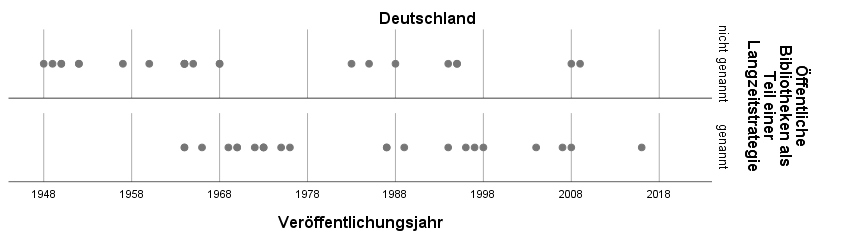
\includegraphics{img/abb_1_de.png} 
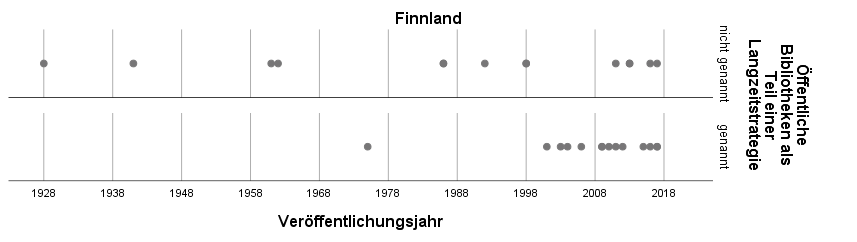
\includegraphics{img/abb_1_fin.png}
\caption{Vorkommen des Themas \enquote{Öffentliche Bibliotheken als Teil einer Langzeitstrategie}}
\end{figure}

\emph{Einheit des Bibliothekssystems}

Durch alle finnischen Papiere hindurch zieht sich das Ziel der
Vereinheitlichung des Bibliothekswesens im ganzen Land. Grundlage
hierfür bilden Angebote und Dienstleistungen, die in allen Bibliotheken
des Landes in gleichbleibender Qualität vorhanden sind, wofür vor allem
kooperativ erstellte Angebote und gut ausgebildetes Personal sorgen
sollen.

\emph{Obligatorischer Masterabschluss für Leitungspositionen}

In Finnland muss die Bibliotheksleitung immer einen Masterabschluss
haben, wohingegen in Deutschland nur für einen kleinen Teil der
Bibliotheken, nämlich ab Sektion 2 (= Öffentliche Bibliothekssysteme und
Bibliotheken für Versorgungsbereiche ab 100.000 Einwohner), ein solcher
erforderlich ist. Sowohl die kooperativen Angebote als auch die
Ausbildung des Personals sind schon in den ersten finnischen
Bibliotheksgesetzen enthalten gewesen und haben dazu geführt, dass man
im ganzen Land vergleichbar gute Öffentliche Bibliotheken findet.

\emph{Obligatorische Evaluation}

Zur Qualitätssicherung gehört in Finnland seit 1998 auch die gesetzlich
vorgeschriebene Evaluation, denn nur mit ihrer Hilfe können die
angebotenen Leistungen auch überprüft werden. Natürlich gibt es auch in
Deutschland Evaluationen, allerdings werden sie von den Bibliotheken
selbst oder deren Trägern initiiert und durchgeführt, eine
Vereinheitlichung der Leistungen aller Bibliotheken wird nicht
angestrebt.

\emph{Gebührenfreiheit}

Die Gebührenfreiheit in Finnland ist ebenfalls eine der Regelungen, die
bereits seit dem ersten Bibliotheksgesetz festgeschrieben wurden. Die
Gebührenfrage wird in Deutschland, wie auch die Rechte und Pflichten der
Benutzer*innen und die Bibliotheksordnung, in die Entscheidungsgewalt
der Bibliotheken beziehungsweise ihrer Träger gelegt, obwohl auch die
deutschen Landesbibliotheksgesetze zumindest überwiegend die
gebührenfreie Vor-Ort-Benutzung vorschreiben.

\emph{Neue und virtuelle Dienstleistungen}

Die Öffentlichen Bibliotheken in Finnland scheinen sich heute stärker
mit neuen Trends und Entwicklungen zu befassen, denn die hybride
Bibliothek beziehungsweise ein gleichberechtigtes Nebeneinander von
physischen und virtuellen Materialien, neue und virtuelle
Dienstleistungen, zeitgemäße Technik und Medienlesefähigkeit tauchen vor
allem oder ausschließlich in neueren finnischen Papieren auf. In
deutschen Papieren wurde in den 1990er Jahren die Einführung von PCs
gefordert. Da die moderne Informationstechnik im Alltag der Menschen
eine wichtige Rolle spielt, müssen auch die Öffentlichen Bibliotheken
entsprechende Angebote und Dienstleistungen vorhalten, um attraktiv zu
bleiben. Weil die Benutzer*innen immer besser ausgebildet sind und gute
Kenntnisse in den neuen Technologien besitzen, muss sich das Personal
entsprechend weiterbilden, um seinen Informationsvorsprung zu bewahren
und den Informationssuchenden in den neuen Medien Hilfestellung bieten
zu können.

\begin{figure}
\centering
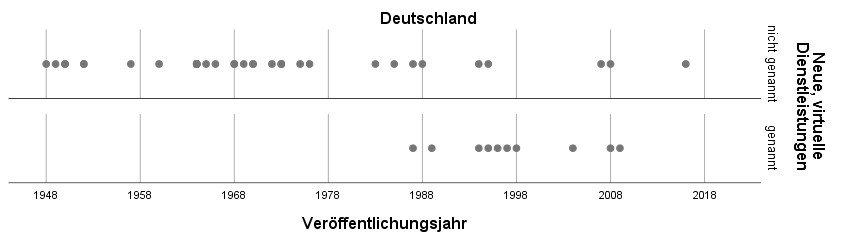
\includegraphics{img/abb_2_de.png} 
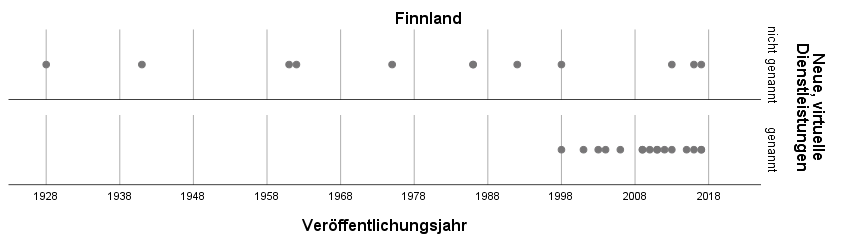
\includegraphics{img/abb_2_fin.png}
\caption{Vorkommen des Themas \enquote{Neue, virtuelle Dienstleistungen}}
\end{figure}

\hypertarget{deutschland-ausstattungsstandards-im-fokus}{%
\subsection{Deutschland: Ausstattungsstandards im
Fokus}\label{deutschland-ausstattungsstandards-im-fokus}}

Die Themen, auf die in deutschen Papieren besonderer Wert gelegt wird,
betreffen vor allem das konkrete Angebot, das Öffentliche Bibliotheken
ihren Benutzer*innen machen sollten, das heißt es werden quantitative
Standards für Bestände, Personal, Gebäude und Einrichtung vorgegeben
sowie Hinweise für Gebäude und zum Bestandsaufbau, was den Bedarf für
unterschiedliche Altersgruppen und unterschiedliche Inhalte angeht.
Diese Veröffentlichungen, die spezifische Ratschläge für das Betreiben
einer guten Bibliothek (wieviel Platz sollte für wie viele Bücher/Medien
welchen Inhalts für welche Benutzergruppe vorhanden sein) beinhalten und
überwiegend im Zeitraum 1964--1973 erschienen sind, zielen
offensichtlich darauf, Bibliotheksvertreter*innen eine
Argumentationshilfe gegenüber Entscheidungsträgern zu geben.

\begin{figure}
\centering
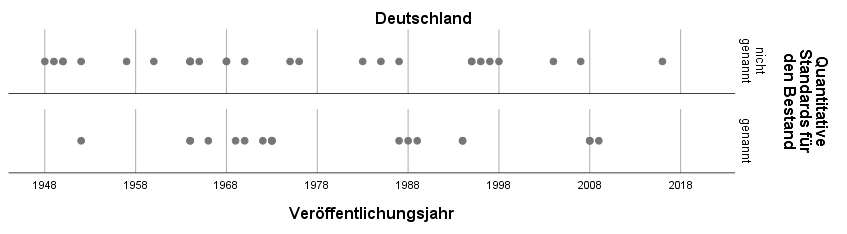
\includegraphics{img/abb_3_de.png} 
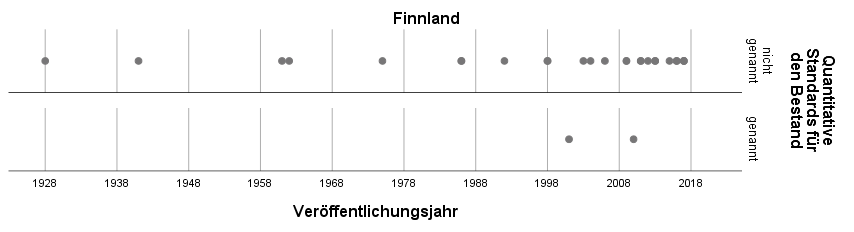
\includegraphics{img/abb_3_fin.png}
\caption{Vorkommen des Themas \enquote{Quantitative Standards für den Bestand}}
\end{figure}


In der finnischen Bibliotheksgesetzgebung werden dagegen beispielsweise
nicht mehr die verschiedenen Medienformate aufgezählt, die den
Bibliotheksnutzer*innen zur Verfügung stehen sollten, sondern es werden
die Dienstleistungen beschrieben, die von Öffentlichen Bibliotheken
angeboten werden sollten, wozu auch das gleichberechtigte Nebeneinander
von Materialien, Sammlungen und Angeboten jeglicher Art passt (Finnland.
Eduskunta 2016, § 6). Eine Erklärung für das Fehlen quantitativer
Standards in den meisten finnischen Papieren könnte sein, dass es schon
seit Anfang der 1960er Jahr in jeder finnischen Gemeinde eine
ausreichend ausgestattete Öffentliche Bibliothek gibt. Eventuell finden
sich entsprechende Vorgaben aber auch in praktischen Handreichungen für
Bibliotheken, die unterhalb der Untersuchungsebene dieses Beitrags
liegen. .

\hypertarget{fazit}{%
\section{Fazit}\label{fazit}}

Trotz der großen Anzahl gleich behandelter Themen in deutschen und
finnischen Papieren wirkt das finnische Öffentliche Bibliothekswesen mit
seinen thematischen Schwerpunkten sehr viel mehr als Einheit als das
deutsche Öffentliche Bibliothekswesen. Alles ist darauf ausgerichtet,
den Benutzer*innen im ganzen Land ein aktuelles, gleichbleibend gutes
Angebot in allen Bereichen anzubieten. Auch in den deutschen
Veröffentlichungen werden Vorschläge für ein einheitliches
Bibliotheksnetzwerk gemacht, wobei man durch die Betonung von
quantitativen Mindeststandards für Ausstattung und Medienangebot den
Eindruck bekommt, dass es eher um die Existenz einzelner Bibliotheken
geht als um die Qualität aller Bibliotheken. Auch das Fehlen einer
übergeordneten Instanz, die verbindliche Regelungen auf nationaler Ebene
festlegt, ist deutlich spürbar, denn natürlich können Ratschläge gemacht
und Hinweise gegeben werden -- diese haben jedoch wenig Wirkung, wenn
ihre Befolgung nicht überprüft oder gefordert werden kann oder
entsprechende finanzielle oder personelle Ressourcen zur Umsetzung durch
mangelnde politische Unterstützung fehlen.

Die Ausgangsfrage, ob ein Grund für den Erfolg der finnischen
Bibliotheken die vorhandene gesetzliche Grundlage ist, würde ich in
jedem Fall mit \enquote{Ja} beantworten, sie ist es aber nicht allein.
Das einheitliche Bild, das sich in der Gesamtheit der finnischen Papiere
zeigt, das \enquote{Ziehen an einem Strang}, um die bestmögliche
Leistung aller Bibliotheken zu erreichen (also eine kooperative Haltung
innerhalb des Berufsstands selbst) hat genauso wie die Anerkennung der
Bedeutung der Öffentlichen Bibliotheken durch die Politik dazu
beigetragen, dass sich das finnische Bibliothekswesen auf der
gesetzlichen Grundlage zu dem entwickelt hat, was es heute ist.

Die Vielzahl der Akteur*innen bei der Planung des deutschen Öffentlichen
Bibliothekswesens erzeugt ein sehr viel diffuseres Bild, obwohl im Laufe
des untersuchten Zeitraums natürlich auch richtungweisende deutsche
Planungspapiere erschienen sind, die aber durch die fehlende gesetzliche
Grundlage und Möglichkeit zur Durchsetzung der Vorschläge keine
einheitliche Entwicklung ermöglichen konnten. Auch in Deutschland gibt
es hervorragende Öffentliche Bibliotheken, gute Netzwerke und innovative
Angebote. Für eine vergleichbare Entwicklung aller Bibliotheken wäre
jedoch mehr politischer Wille nötig, um doch zumindest eine gemeinsame
nationale Bibliothekspolitik auf die Beine zu stellen, wofür auch eine
nationale Planungseinheit nützlich wäre. Der deutsch-finnische Vergleich
zeigt, dass das Zusammenwirken aller Akteure immer noch das beste Ziel
erreicht -- Absichtserklärungen einzelner Teile des Systems können
hingegen ohne Wirkung bleiben.

\hypertarget{literatur}{%
\section{Literatur}\label{literatur}}

Deutsche Bibliothekskonferenz; Deutscher Büchereiverband; Arbeitsstelle
für das Büchereiwesen (1973): \emph{Bibliotheksplan 1973. Entwurf eines
umfassenden Bibliotheksnetzes für die Bundesrepublik Deutschland}.
Berlin: Dt. Bibliothekskonferenz.

Europarat (2000): \emph{Bibliotheksgesetzgebung und -politik in Europa.
Richtlinien} {[}12.10.1999{]}. In: Bibliotheksgesetzgebung in Europa.
Diskussionsbeiträge und Länderberichte. Hrsg. von Christiane Bohrer. Bad
Honnef: Bock + Herchen (Bibliothek und Gesellschaft), S. 27--35.

Finnland. Opetus- ja Kulttuuriministeriö (2006): \emph{Library
development program 2006--2010. The library as an integrated service
center for rural and urban areas}. Helsinki.

Finnland. Opetusministeriö (2003): \emph{Bibliothekenstrategie 2010.
Politik des Bildungsministeriums zur Sicherstellung des Zugangs zu
Wissen und Kultur. Öffentliche Bibliotheken in Finnland}. Helsinki.
(Veröffentlichungen des Bildungsministeriums 39).

Herde, Sari (2019): \emph{Grundsätzlich besser? Finnlands nationale
Konzepte, Strategien und Empfehlungen für Bibliotheken}. Masterarbeit.
Berlin: HU Berlin, Institut für Bibliotheks- und
Informationswissenschaft.

IFLA (1956): \emph{Die Entwicklung des Öffentlichen Bibliothekswesens.
IFLA-Memorandum}. -- In: Bücherei und Bildung 7, S. 239--247.

IFLA; UNESCO (2005): \emph{Dienstleistungen Öffentlicher Bibliotheken.
IFLA/UNESCO Richtlinien für die Weiterentwicklung}. München: K.G. Saur.

Thauer, Wolfgang; Vodosek, Peter (1990): \emph{Geschichte der
öffentlichen Bücherei in Deutschland}. 2. Aufl. Wiesbaden: Harrassowitz.

UNESCO (1979): \emph{Unesco public library manifesto}. In: Unesco
journal of information science, librarianship and archives
administration Vol. 1, No.~4, S. 230--232.

Volpers, Helmut (2013): \emph{Inhaltsanalyse}. In: Handbuch Methoden der
Bibliotheks- und Informationswissenschaft. Bibliotheks-,
Benutzerforschung, Informationsanalyse. Hrsg. von Konrad Umlauf, Michael
S. Seadle u.a. Berlin, Boston: De Gruyter Saur.

\hypertarget{gesetze-und-verordnungen}{%
\subsection{Gesetze und Verordnungen}\label{gesetze-und-verordnungen}}

Finnland. Eduskunta (1928): \emph{Kansankirjastolaki 131/1928}.

Finnland. Eduskunta (1961): \emph{Kirjastolaki 235/1961}.

Finnland. Eduskunta (1986): \emph{Kirjastolaki 235/1986}.

Finnland. Eduskunta (1998): \emph{Kirjastolaki 904/1998}.

Finnland. Eduskunta (2016): \emph{Laki yleisistä kirjastoista
1492/2016}. (Englische Übersetzung:
\url{https://www.finlex.fi/en/laki/kaannokset/2016/20161492}), zuletzt
geprüft am 23.3.2020

Finnland. Opetus- ja Kulttuuriministeriö (2017): \emph{Opetus- ja
kulttuuriministeriön asetus yleisistä kirjastoista 660/2017}.

Finnland. Opetusministeriö (1928): \emph{Asetus kansankirjastoista
144/1928}.

%autor
\begin{center}\rule{0.5\linewidth}{0.5pt}\end{center}

\textbf{Sari Herde} hat Finnougristik an der Universität Hamburg
studiert und ist seit 2002 Fremdsprachenassistentin in der
Osteuropa-Abteilung der Staatsbibliothek zu Berlin. Berufsbegleitendes
Fernstudium der Bibliotheks- und Informationswissenschaft am IBI der HU
Berlin von 2017-2019.

\end{document}
